
%%% Local Variables:
%%% mode: latex
%%% TeX-master: "section02.tex"
%%% End:
%%%%%%%%%%%%%%%%%%%%%%%%%%%%%%%%%%%%%%%%%%%%%%%%%%%%%%%%%%%%
\section{统计绘图工具}
%%%%%%%%%%%%%%%%%%%%%%%%%%%%%%%%%%%%%%%%%%%%%%%%%%%%%%%%%%%%
\subsection{为什么用绘图工具}
\begin{frame}{\subsecname}{}

  \begin{columns}
    \begin{column}{.5\textwidth}
      \begin{figure}
        \centering 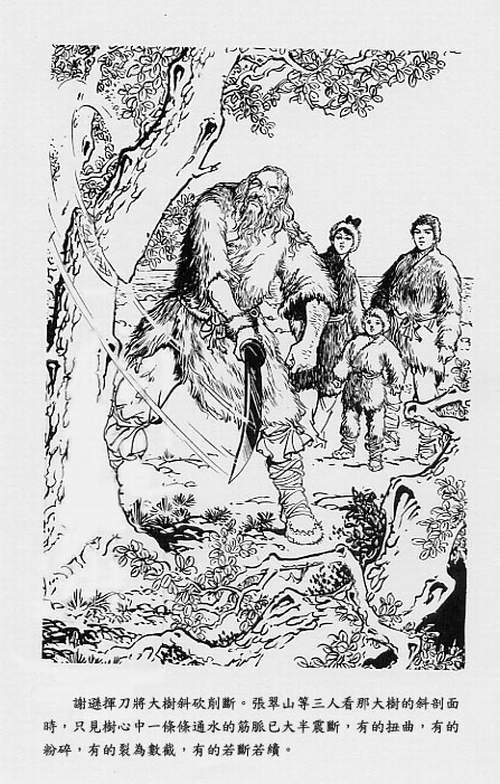
\includegraphics[width=0.9\columnwidth]{屠龙宝刀.jpg}
      \end{figure}
    \end{column}

    \begin{column}{.48\textwidth}
      \begin{ornamentblock}
        \centering
        {工欲善其事,必先利其器\\
          \rightline{\textemdash《论语·卫灵公》}}
      \end{ornamentblock}
      % \curlyframe{工欲善其事,必先利其器\\
      % \rightline{-----《论语·卫灵公》}}
    \end{column}
  \end{columns}

\end{frame}

\begin{frame}[c]{\subsecname}
  
  \begin{columns}
    \begin{column}{.6\textwidth}
      \begin{figure}
        \centering 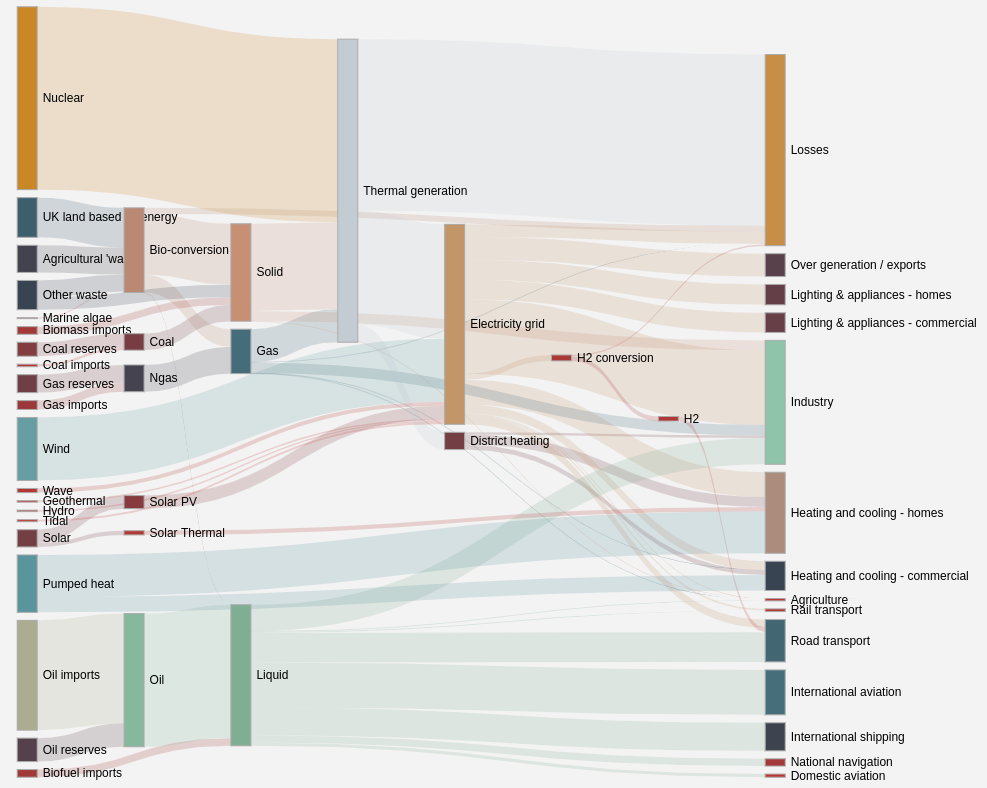
\includegraphics[width=\columnwidth]{sankey.png}
        \caption{看上去复杂但是直观的桑基图(Sankey diagram)}
      \end{figure}
    \end{column}

    \begin{column}{.4\textwidth}
      \begin{block}{直观与简单} \small
        \begin{itemize}
        \item[\HandRight] \emphText{统计量是统计图形最关键的构成因素},
        因此,优秀的统计图形背后必然隐藏着重要的统计量
        \item[\HandRight] 图形的首要作用是“直观”展示统计量信息,
        但是\emphText{能够直观理解的信息未必是“简单”的}
        \item[\HandRight] 使用合适的工具可以让信息的表达既“直观”又“简单” 
        \end{itemize}
      \end{block}
    \end{column}
  \end{columns}
    
\end{frame}

\subsection{何为利器}
\begin{frame}[t]{\subsecname}
  \begin{itemize}
    \item 统计计算功能齐全
    \item 图形元素易于控制
    \item 统计图形种类丰富
  \end{itemize}

\begin{figure}[ht]
  \centering 
\includegraphics[width=0.8\textwidth]{stat_tools.png}
  \caption{常见的一些统计绘图工具}
\end{figure}
\end{frame}

\subsection{所见即所得工具}

\begin{frame}[t]{\subsecname}{excel}
\begin{itemize}
\item<1-> 微软公司开发的电子数据表软件,从1985年发布1.0版本
    至今已经30多年历史,是电子数据表类软件的工业标准
\item<2-> 优秀的人机实时交互设计,所见即所得
\item<3-> 能够完成简单的统计功能以及数据绘图,但并不是统计软件
\end{itemize}

\begin{overlayarea}{\textwidth}{\textheight} 
  \only<1>{
    \begin{figure}\centering
      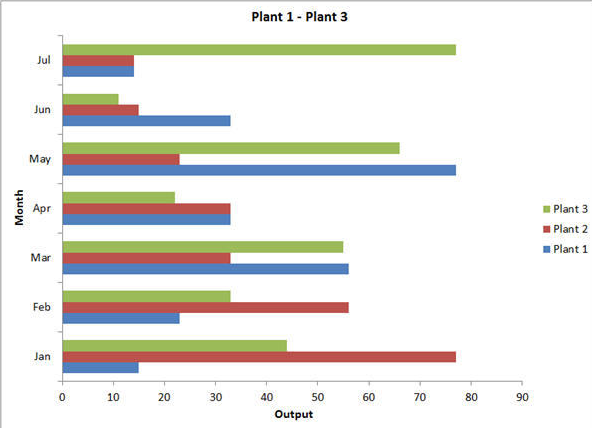
\includegraphics[width=0.65\columnwidth] {excel条形图.png}
      \caption{表示绝对数值大小的条形图}
    \end{figure}}

  \only<2>{
    \begin{figure}\centering
      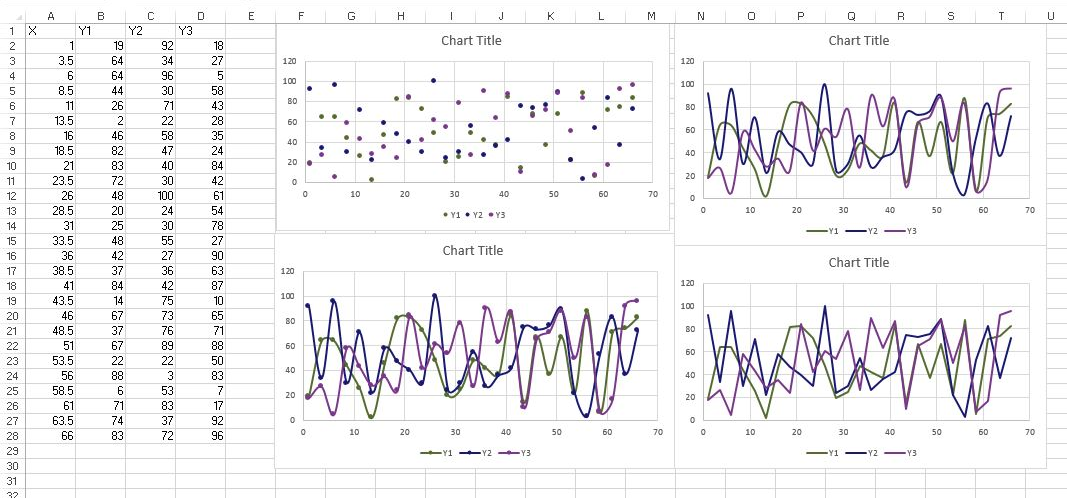
\includegraphics[width=\columnwidth] {excel折线图.png}
      \caption{表示绝对数值大小的折线图}
    \end{figure}}
  
  \only<3>{
    \begin{figure}[ht]
      \centering 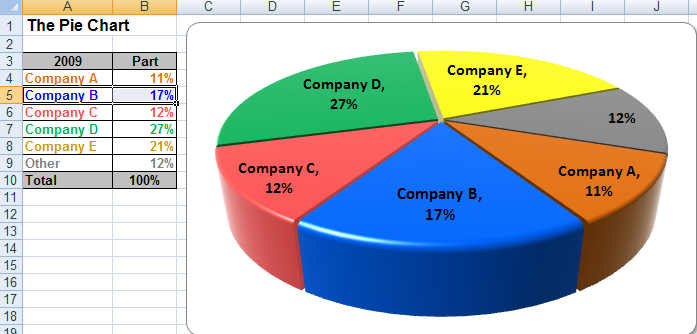
\includegraphics[width=\columnwidth]{excel饼图.png}
      \caption{表示比例大小的饼图}
    \end{figure}}

  \only<4>{
    \begin{figure}[ht]
      \centering 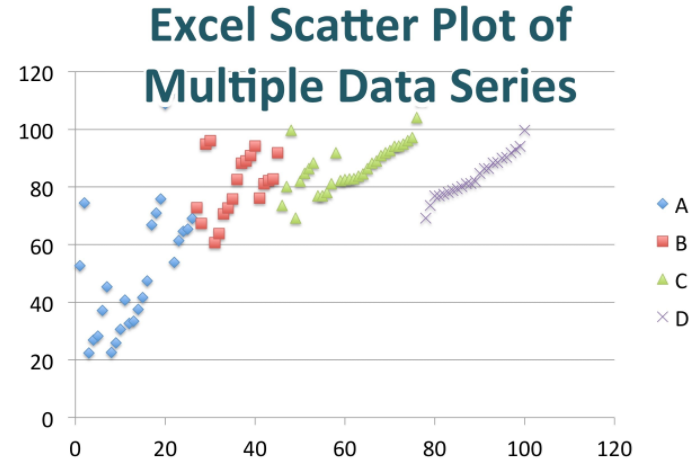
\includegraphics[width=0.7\columnwidth]{excel散点图.png}
      \caption{表示二维变量关系的散点图}
    \end{figure}}
   
  \only<5->{
    \begin{alertblock}{excel作为统计绘图工具的缺点}
      \begin{itemize} \small
        \item<6-> [\PencilLeftDown] excel并非专业统计软件,只擅长对原始数据的展示,统
        计分析和建模功能十分有限。因此,著名统计学家Leland
        Wilkinson\footnotemark[1] 说\emphText{“给统计刊物投稿时永远不要用Excel作图”}
        \item<7->[\PencilLeftDown] 只能在windows单机上运行,处理数据量有限而且速度慢,
                 不具备大规模数据管理功能
        \item<8->[\PencilLeftDown] 绘图功能十分有限,只提供部分基本统计图形 
      \end{itemize}
    \end{alertblock}
~} %使footnote看上去在“最下面”
\only<6->{
\footnotetext[1]{统计学经典书籍《The Grammar of Graphics》一书的作者,任职SPSS公司十年,而且一直领导其可视化小组}}
\end{overlayarea}  

% \renewcommand{\footnoterule}{}
% \uncover<6->{\footnoterule}

\end{frame}

\begin{frame}[t]{\subsecname}{SPSS}
  \begin{itemize}
    \item<1-> 易学易用
    \item<2-> 功能全面
    \item<3-> 界面友好
  \end{itemize}

\begin{overlayarea}  {\textwidth}{\textheight}
  \only<1-3>{
    \begin{figure}[ht]
      \centering 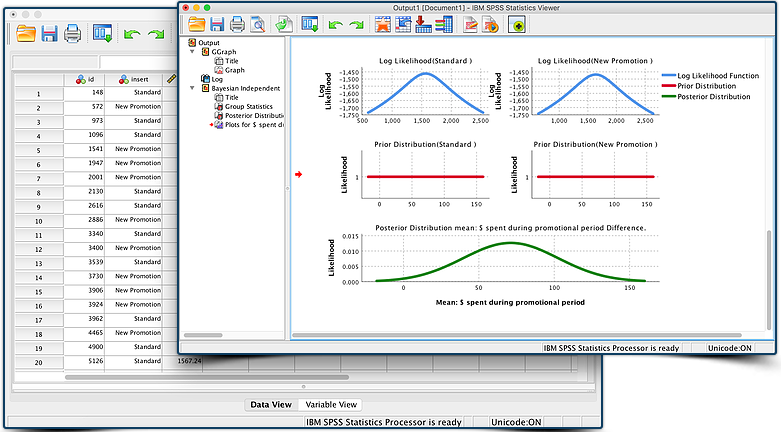
\includegraphics[width=0.9\textwidth]{SPSS.png}
      \caption{SPSS用户操作界面}
    \end{figure}}
   
  \only<4->{
    \begin{alertblock}{SPSS及其他所见即所得工具的缺陷}
      \begin{itemize} \small
        \item<4->[\PencilLeftDown] 按钮的数量总是有限的,而统计模型是无限的
        \item<5->[\PencilLeftDown] 计算机完成了太多图形要素控制工作,缺乏灵活性
        \item<6->[\PencilLeftDown] 生成一张图易,生成N张图难
        \item<7->[\PencilLeftDown] 贫穷限制了想象力:商业软件费用高昂,而且部分模块需单独付费
      \end{itemize}
    \end{alertblock}}
\end{overlayarea}
\end{frame}

\subsection{所想即所得工具}
\begin{frame}[t]{\subsecname}{SAS}
  \begin{itemize}
    \item<1-> 1960年诞生于SAS软件研究所,老牌专业统计软件
    \item<2-> 基于数据库进行数据管理,具有大型数据集处理分析能力
    \item<3-> 有专门的SAS认证考试,包括程序员、业务分析师、数据挖掘、系统开发
           专家和系统管理专家五种不同角色
  \end{itemize}
  
  \begin{overlayarea} {\textwidth}{\textheight}
    \only<1-4>{
      \begin{figure}
        \centering 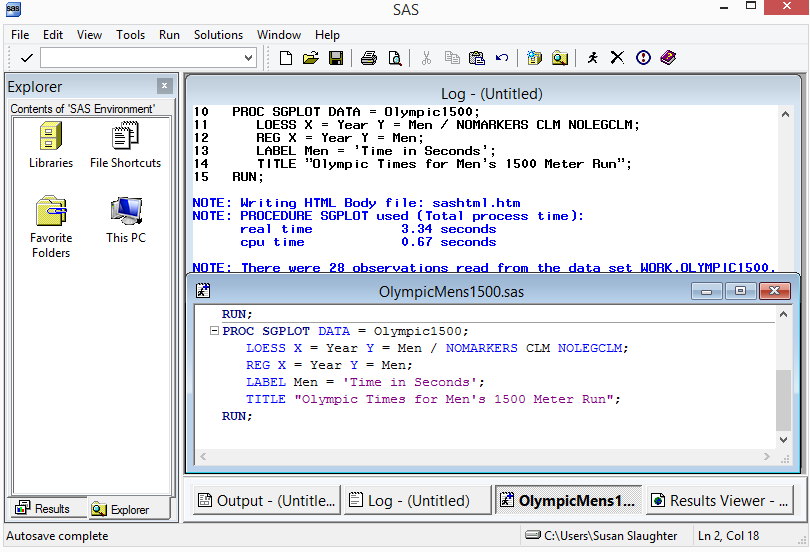
\includegraphics[width=0.7\columnwidth]{sas_ui.png}
        \caption{SAS软件界面}
      \end{figure}}
  \end{overlayarea}
\end{frame}

\begin{frame}[t, fragile]{\subsecname}{SAS}
  \begin{itemize}
    \item 200多个集成模块,涵盖了主流统计模型和分析方法,而且通过内置
           脚本语言实现统计建模和绘图等功能
  \end{itemize}
 
      \begin{columns}
        \begin{column}[c]{.5\textwidth}
          \centering 
          \begin{figure}
            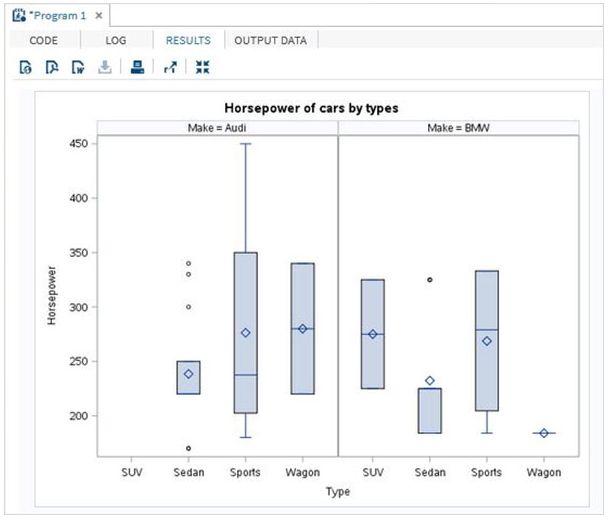
\includegraphics[width=0.8\columnwidth]{sas_boxplot.png}
            \caption{箱形图(Box plot)}
          \end{figure}
        \end{column}

        \begin{column}[c]{.5\textwidth}\centering
\begin{lstlisting}[language=SAS]
PROC SQL;
create table CARS1 as
SELECT make,model,type,invoice,horsepower,length,weight
 FROM SASHELP.CARS
WHERE make in ('Audi','BMW');
RUN;

PROC SGPLOT  DATA=CARS1;
  VBOX horsepower 
  / category = type;

   title 'Horsepower of cars by types';
RUN; 
\end{lstlisting}
        \end{column}
      \end{columns}
\end{frame}

\begin{frame}[t]{\subsecname}{S-Plus}
    \begin{itemize}
      \item S语言是1976年AT\&T贝尔实验室开发的一种用于统计计算的解释型编程语言
    \end{itemize}

    \begin{figure}
      \centering 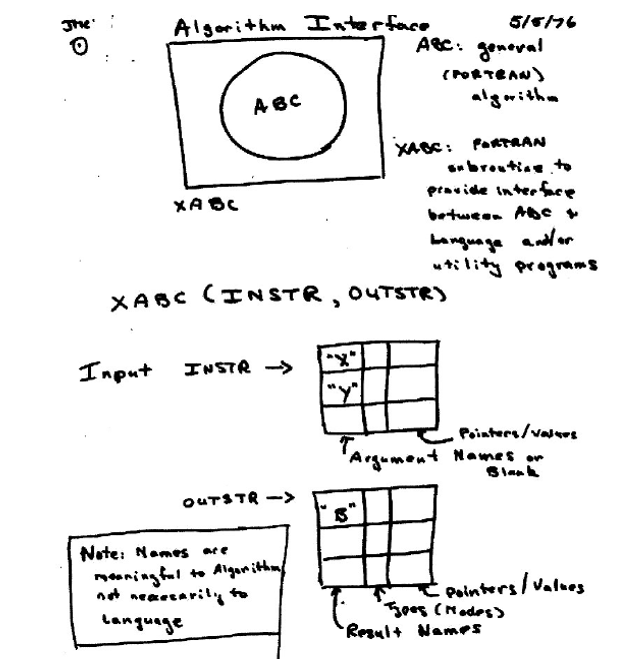
\includegraphics[width=0.5\columnwidth]{S_init.png}
      \caption{S语言的设计草图(1976.5.5)}
    \end{figure}

\end{frame}   

\begin{frame}[t, fragile]{\subsecname}{S-Plus}
    \begin{itemize}
      \item 与SAS内置脚本语言相比,S语言更加符合现代程序语言的设计,方便灵活控制
            图形输出,制作既精美又专业的统计图形
      \item 能够与其他主流程序语言集成
    \end{itemize}

    \begin{onlyenv}<1>
      \begin{columns}
        \begin{column}{.7\textwidth}
          \begin{figure}
            \centering
            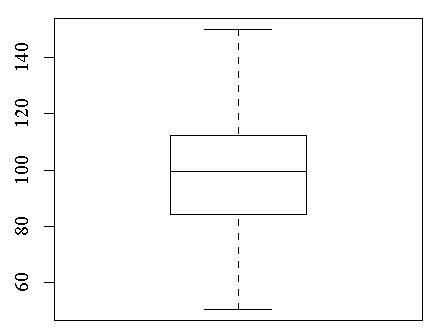
\includegraphics[width=0.8\columnwidth]{splus_boxplot.png}
            \caption{箱形图(Box plot)}
          \end{figure}
        \end{column}

        \begin{column}{.3\textwidth}
\begin{lstlisting}[language=S]
  boxplot(Weight)
\end{lstlisting}
        \end{column}
      \end{columns}
    \end{onlyenv}
\end{frame}    

\begin{frame}[t]{\subsecname}{S-Plus}
    \begin{itemize}
      \item S-Plus是基于S语言开发的商业化统计软件,1993年由MathSoft公司开发,
            2008年起由TIBCO负责运维
      \item 与SPSS和SAS并称世界三大统计软件,具有专业的统计功能
    \end{itemize}

    \begin{figure}
      \centering 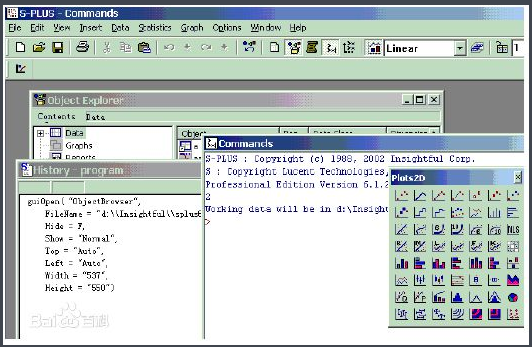
\includegraphics[width=0.8\columnwidth]{splus_ui.png}
      \caption{S-Plus软件界面}
    \end{figure}
\end{frame}    

\begin{frame}{\subsecname}{}
  % \begin{variableblock}{所想即所得工具}{bg=green!20,fg=black}{fg=white,bg=SpringGreen4}
  %   \begin{itemize}
  %   \item wowo
  %   \item sdsfs
  %   \end{itemize}
  % \end{variableblock}
\onslide<1->{
  \begin{goodbox}{所想即所得工具的优势}
     \begin{itemize}
     \item[\PencilLeftDown] 想象力有多大,世界就有多精彩
     \item[\PencilLeftDown] 花有重开日,人无再少年
     \item[\PencilLeftDown] 深入算法内核,由术至道 
     \end{itemize}
  \end{goodbox}}

\onslide<2->{
  \begin{badbox}{所想即所得工具的劣势}
     \begin{itemize}
     \item[\PencilLeftDown] 人机交互全靠指令输入,需要具备编程基础
     \item[\PencilLeftDown] 需要扎实的统计学基础,学习曲线陡峭
     \item[\PencilLeftDown] 实现简单的统计功能时不如“所见即所得工具”快捷    
     \end{itemize}
  \end{badbox}}

\end{frame} 
